\begin{problem}{\problemnum \, \textsf{(POOLE 1.1.22)}}
	Draw the standard coordinate axes on the same diagram as the axes relative to $\bu$ and $\bv$.
	Use these to find $\bw$ as a linear combination of $\bu$ and $\bv$.
	\[ \bu = \begin{pmatrix} -2 \\ 3 \end{pmatrix},
	   \bv = \begin{pmatrix}  2 \\ 1 \end{pmatrix},
	   \bw = \begin{pmatrix}  2 \\ 9 \end{pmatrix}
	\]
\end{problem}
\begin{solution}\\\\
\begin{center}
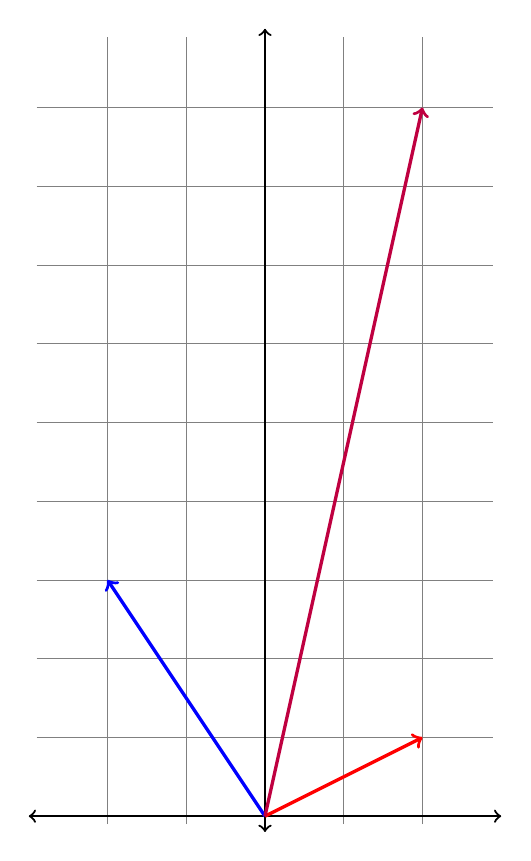
\begin{tikzpicture}
	% grid
	\draw[step=1cm, gray, very thin] (-2.9,-.1) grid (2.9, 9.9);

	% x axis
	\draw[thick, <->] (-3,0) -- (3,0);

	% y axis
	\draw[thick, <->] (0, -.2) -- (0, 10);

	% u vector
	\draw[very thick, color=blue, ->] (0, 0) -- (-2, 3);

	% v vector
	\draw[very thick, color=red, ->] (0, 0) -- (2, 1);

	% w vector
	\draw[very thick, color=purple, ->] (0, 0) -- (2, 9);
\end{tikzpicture}\end{center}
\[ 2{\color{blue}\bu} + 3{\color{red}\bv} = {\color{purple}\bw} \]
\end{solution}
